% !TEX root = main.tex

\section{语义分析与中间表示}
\begin{itemize}
\item 高层中间表示:语法树、有向无环图(DAG),用于静态类型检查
\item 低层中间表示:三地址码,适合机器相关的任务(寄存器分配、指令选择)
\end{itemize}
\begin{lstlisting}[language=c++]
x = y op z // arithmetic and logical
x = op y  // negation and conversion
x = y // copy
goto L // unconditional jump
if x goto L // conditional jump 
if False x goto L // conditional jump
if x op y goto L // relational operation
param x1 // parameter passing
param x2
...
param xn
call p, n // procedure call
y = call p, n // function call
return y // return a value
x = y[i] // indexed copy, i is the offset
x[i] = y
x = &y // address and pointer assignment
x = *y
*x = y
\end{lstlisting}

\verb'top'指代当前的符号表,\verb'gen'代表生成中间代码,\verb'||'代表代码的连接,\verb'next'定义执行完$S$之后紧跟的指令。
\begin{center}
\begin{tabular}{|l|l|}\hline
$S \to id = E$ & \verb"S.code = E.code || gen(top.get(id.lexeme) '=' E.addr)"\\\hline
$E \to E_1 + E_2$ & \begin{tabular}{l}
\verb'E.addr = new Temp()'\\
\verb"E.code = E1.code || E2.code || gen(E.addr '=' E1.addr '+' E2.addr)"
\end{tabular}\\\hline
$E \to -E_1$ & \begin{tabular}{l}
\verb'E.addr = new Temp()'\\
\verb"E.code = E1.code || gen(E.addr '=' minus E1.addr)"
\end{tabular}\\\hline
$E \to (E_1)$ & \begin{tabular}{l}
\verb'E.addr = E1.addr'\\
\verb"E.code = E1.code"
\end{tabular}\\\hline
$L \to L_1 [E]$ & \begin{tabular}{l}
\verb'L.array = L1.array'\\
\verb"L.type = L1.type.element"\\
\verb"t = new Temp()"\\
\verb"L.addr = new Temp()"\\
\verb"gen(t '=' E.addr '*' L.type.width)"\\
\verb"gen(L.addr '=' L1.addr '+' t)"
\end{tabular}\\\hline
\verb'S'$\to$\verb'if (B) S1 else S2' & \begin{tabular}{l}
\verb'B.true = new Label()'\\
\verb'B.false = new Label()'\\
\verb'S1.next = S2.next = S.next'\\
\verb'S.code = B.code || label(B.true) || S1.code ||'\\
\verb"         gen('goto' S.next) || label(B.false) || S2.code"
\end{tabular}\\\hline
\end{tabular}
\end{center}

三地址码与对应的DAG如下图所示,注意这里将相同终端符号结点都给合并了。

\begin{minipage}{0.5\linewidth}
\[\begin{aligned}
t_1 &= b - c\\
t_2 &= a * t_1\\
t_3 &= a + t_2\\
t_4 &= t_1 * d\\
t_5 &= t_3 + t_4
\end{aligned}\]
\end{minipage}
\begin{minipage}{0.5\linewidth}
\begin{figure}[H]
\centering
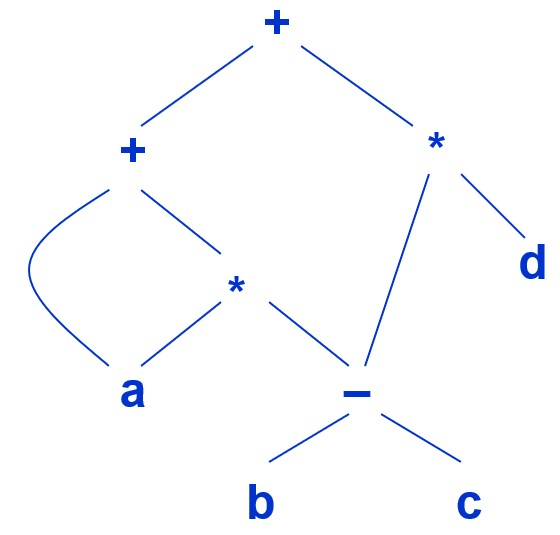
\includegraphics[width=0.5\linewidth]{fig/three-addr-code-dag.jpg}
\end{figure}
\end{minipage}

\begin{example}
令\verb'a'表示一个$2\times 3$的整型数组,\verb'b'表示一个$3\times 4$的整型数组.
假定一个整数的宽度为$4$.
试使用课本图6.22的翻译模式,翻译赋值语句\verb'x=a[i][j]+b[i][j]'.
提示:参考课本例6.12.
\end{example}
\begin{analysis}
带注释的分析树如下
\begin{center}
\scalebox{0.8}{
\begin{forest}
sn edges
[{$S$}
	[{$x$}]
	[{$=$}]
	[{$E.addr=t_9$}
		[{$E.addr=t_4$}
			[{\begin{tabular}{l}$L.array=a$\\ $L.type=int$\\ $L.addr=t_3$\end{tabular}}
				[{\begin{tabular}{l}$L.array=a$\\ $L.type=array(3,int)$\\ $L.addr=t_1$\end{tabular}}
					[{\begin{tabular}{l}$a.type=$\\$array(2,array(3,int))$\end{tabular}}]
					[{$[$}]
					[{$E.addr=i$}
						[{$i$}]
					]
					[{$]$}]
				]
				[{$[$}]
				[{$E.addr=j$}
					[{$j$}]
				]
				[{$]$}]
			]
		]
		[{$+$}]
		[{$E.addr=t_8$}
			[{\begin{tabular}{l}$L.array=b$\\ $L.type=int$\\ $L.addr=t_7$\end{tabular}}
				[{\begin{tabular}{l}$L.array=b$\\ $L.type=array(4,int)$\\ $L.addr=t_5$\end{tabular}}
					[{\begin{tabular}{l}$b.type=$\\$array(3,array(4,int))$\end{tabular}}]
					[{$[$}]
					[{$E.addr=i$}
						[{$i$}]
					]
					[{$]$}]
				]
				[{$[$}]
				[{$E.addr=j$}
					[{$j$}]
				]
				[{$]$}]
			]
		]
	]
]
\end{forest}
}
\end{center}

生成的三地址码如下
\begin{center}
\begin{tabular}{l}
$t_1 = i * 12$\\
$t_2 = j * 4$\\
$t_3 = t_1 + t_2$\\
$t_4 = a[t_3]$\\
$t_5 = i * 16$\\
$t_6 = j * 4$\\
$t_7 = t_5 + t_6$\\
$t_8 = b[t_7]$\\
$t_9 = t_4 + t_8$\\
$x   = t_9$
\end{tabular}
\end{center}
\end{analysis}

注意区别语法分析树(parse tree)和抽象语法树(AST),前者从CFG得到,后者直接由源码得到。
下面例子源自\href{https://en.wikipedia.org/wiki/Abstract_syntax_tree}{Wiki}。
\begin{lstlisting}
while b != 0
  if a > b
    a = a - b
  else
    b = b - a
return a
\end{lstlisting}
\begin{figure}[H]
\centering
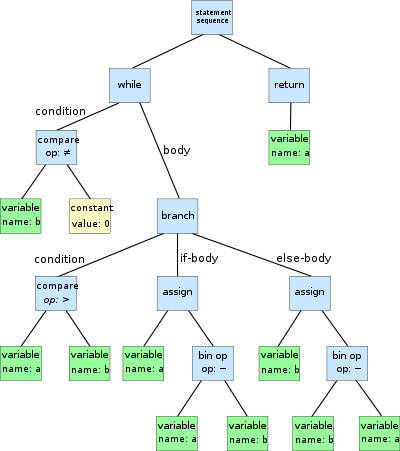
\includegraphics[width=0.5\linewidth]{fig/AST.png}
\end{figure}